\documentclass[11pt]{article}

\usepackage[review]{acl}
\usepackage{times}
\usepackage{latexsym}
\usepackage[T1]{fontenc}
\usepackage[utf8]{inputenc}
\usepackage{microtype}
\usepackage{inconsolata}
\usepackage{graphicx}
\usepackage{booktabs}
\usepackage{multirow}

\title{When RAG Evaluation Fails Silently:\\
Judge Overflow, Context-Filter Interactions, and Passage-Level Recall Blind Spots}

\author{Anonymous ACL submission}

\begin{document}
\maketitle

\begin{abstract}
We report three evaluation and grounding failures discovered while running a controlled, replicated ablation of a local retrieval-augmented generation (RAG) pipeline over 60 hand-written questions on 12 RAG papers.
First, an LLM-as-judge silently returns schema-valid zero scores once its input context exceeds ${\sim}$2,500 tokens, producing apparent pipeline collapses (${\sim}$10/100) that are evaluation artifacts rather than generation failures; after diagnosis and a context cap, affected conditions still regress substantially ($-$19.1 and $-$17.3 points for top-$k{=}10$ and 512-word chunks).
Second, a naive post-reranking sentence filter---motivated by learned context filtering \citep{wang2023filco}---costs 14.3 points when restricted to five sentences per chunk, with context recall falling 23.6 points despite unchanged retrieval.
Third, document-level Recall@5 remains 100\% on a question where PDF chunking splits the answer across a boundary, masking a passage-level failure that only surfaced under faithful generation.
We release all 66 ablation runs (three replications per condition) with pre- and post-fix judge scores; code and data in an anonymized repository (link upon acceptance).
\end{abstract}

\section{Introduction}

Retrieval-augmented generation (RAG) pipelines combine interchangeable components---retrievers, rerankers, context filters, and generators---each with hyperparameters that affect whether a model can ground answers in retrieved evidence \citep{lewis2020rag,gao2023survey}.
End-to-end benchmarks \citep{chen2024rgb,es2024ragas} and best-practice studies \citep{wang2024bestpractices,li2025bestpractices} typically report aggregate scores over fixed configurations, but iterative development often stacks multiple edits between measurements, and evaluation itself can mislead when judges or metrics fail silently.
Unlike these aggregate comparisons, we isolate single-variable effects with three replications per condition against a locked baseline.

We built a fully local RAG pipeline (Qdrant, Ollama, consumer GPU), locked its best configuration (composite score 83.22 on our development set), and ran nine single-variable ablations with three replications each---66 runs total, every condition complete.
Rather than catalog all nine components, this short paper focuses on three findings that bear directly on \emph{faithful} RAG evaluation: an LLM-judge context-overflow failure mode, a destructive interaction between reranking and heuristic context filtering, and a passage-level blind spot in document-level recall.
We treat expected effects (larger generators help, rerankers help, smaller chunks help) as background; the complete 21-condition grid and run artifacts are available in an anonymized repository (link upon acceptance).

\section{Experimental Setup}

\paragraph{Corpus and questions.}
Our evaluation corpus comprises 12 recent RAG papers on query rewriting, self-RAG, context filtering, and related topics indexed into 558 word-based chunks (256 words, 50 overlap).
We hand-wrote five questions per paper (60 total); \texttt{expected\_source} is the gold PDF filename.
This self-built benchmark risks convenience bias (Section~\ref{sec:limitations}); we use it to stress-test our own pipeline, not as a community benchmark.

\paragraph{Locked baseline.}
Hybrid BM25+dense retrieval (BGE-small; \citealt{xiao2024bge}), BGE cross-encoder reranking, no context filter, Qwen2.5-14B generation under a strict JSON schema with deterministic citation parsing, and a separate Qwen2.5-14B judge.
Final score is a weighted composite: 0.35 answer correctness + 0.25 faithfulness + 0.20 context recall + 0.10 context precision + 0.10 citation accuracy; the first four are LLM-judged, citation accuracy is deterministic.
We additionally track Recall@5 (binary, \emph{document}-level).

\paragraph{Ablation protocol.}
Each ablation changes one variable from the locked baseline with $n{=}3$ replications.
Three replications of the unchanged baseline yield mean 81.79 ($\sigma{=}1.52$), which we use as a practical noise floor---not a formal significance test (Section~\ref{sec:limitations}).
Mid-study we discovered a judge failure (Section~\ref{sec:judge}); we capped judge input at five chunks / 1,920 words while the generator still receives full top-$k$ context, re-ran affected conditions, and archive pre-fix scores.

\section{Findings}

\subsection{LLM-Judge Context Overflow}
\label{sec:judge}

Ablation~8 (retrieval depth) and Ablation~9 (chunk size) initially appeared catastrophic.
With top-$k{=}10$ or 512-word chunks, mean final scores were 9.9 and 14.1 (Table~\ref{tab:judge-fix})---the kind of collapse that invites a reviewer to distrust the entire pipeline.
Yet JSON parse rate stayed at 100\% and deterministic citation accuracy remained near 80\%; generation was not failing wholesale.

The judge, however, returned schema-valid JSON with all four LLM-scored fields set to zero once its input exceeded roughly 2,500 tokens (${\sim}$2,560 words in our top-$k{=}10$ runs).
Only citation accuracy (${\sim}$10\% of the composite) contributed, yielding scores of 8--14.
Re-judging stored outputs with capped context immediately recovered per-question scores of 50--80.
We implemented \texttt{JUDGE\_MAX\_CONTEXT\_CHUNKS=5} and \texttt{JUDGE\_MAX\_CONTEXT\_WORDS=1920} in our scoring module and re-ran both conditions.

Post-fix means are 64.1 ($\sigma{=}2.1$) for top-$k{=}10$ and 65.9 ($\sigma{=}0.9$) for chunk-512---still large regressions ($-$19.1 and $-$17.3 vs.\ baseline 83.22), but now attributable to context dilution at generation time rather than judge failure.
Top-$k \in \{5,7\}$ and chunk sizes 128/256 remain within or just outside the noise band (Table~\ref{tab:key-results}).
This failure mode is especially dangerous because silent zeros look like genuine poor grounding; nothing in a results table flags them as bugs.
Any RAG evaluation that pipes variable-length retrieved context into an LLM judge is exposed.

\begin{table}[t]
  \centering
  \small
  \begin{tabular}{lccc}
    \toprule
    \textbf{Condition} & \textbf{Pre-fix} & \textbf{Post-fix} & \textbf{$\Delta$} \\
    \midrule
    A8 top-$k{=}10$ & 9.9 & 64.1 $\pm$ 2.1 & $-$19.1 \\
    A9 chunk 512 & 14.1 & 65.9 $\pm$ 0.9 & $-$17.3 \\
    \bottomrule
  \end{tabular}
  \caption{Judge overflow artifact vs.\ corrected scores (means over 3 runs; $\Delta$ vs.\ baseline 83.22). Pre-fix archives retained for audit.}
  \label{tab:judge-fix}
\end{table}

\begin{figure}[t]
  \centering
  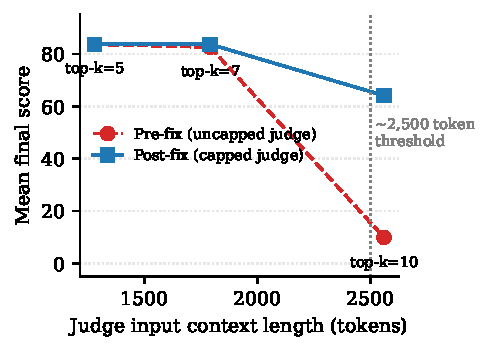
\includegraphics[width=\columnwidth]{fig1_judge_overflow.pdf}
  \caption{Mean final score vs.\ judge input context length (A8 top-$k$).
  Pre-fix scores collapse past the ${\sim}$2,500-token threshold; post-fix (capped) scores reveal the true regression from context dilution at generation time.}
  \label{fig:overflow}
\end{figure}

\subsection{Post-Reranking Context Filter Regression}
\label{sec:filter}

Ablation~4 tests a heuristic sentence filter applied \emph{after} cross-encoder reranking: keep the top 10 or top 5 sentences from each retrieved chunk.
This is inspired by learned context filtering \citep{wang2023filco} but uses a fixed rule rather than a trained selector.

The filter interacts badly with reranking (Table~\ref{tab:key-results}).
With no filter, mean final score is 82.9 ($\sigma{=}1.0$), within noise of baseline.
Top-10 sentences costs 4.2 points (78.99); top-5 sentences costs \textbf{14.3 points} (68.9, $\sigma{=}0.5$)---the largest controlled effect among settings that do not change how many chunks reach the generator.
Context recall drops from 86.4 to 62.8 ($-$23.6); answer correctness from 79.4 to 63.5.
Our own development trajectory had bundled this filter with other changes in an earlier run (67.1 $\rightarrow$ 83.2 when disabled); the ablation isolates the filter as the dominant regression.

Reranking surfaces high-scoring but sentence-sparse chunks; truncating to five sentences then removes the evidence the reranker selected.
Learned filters may succeed where fixed heuristics fail, but our result warns against assuming post-reranking truncation is safe.

\subsection{Document Recall Masks Passage-Level Failure}
\label{sec:recall}

Question \texttt{adaptllm\_q5} asks for the main bottleneck in ADAPT-LLM performance; the answer states that information retrieval is the bottleneck, supported by gold-vs.-retrieved passage comparisons.
Across 12+ full-pipeline runs with hybrid retrieval, Recall@5 is \textbf{100\%}---the correct PDF is always retrieved---yet final score is \textbf{10.0} whenever the generator correctly refuses to answer from insufficient context.

Diagnosis: \texttt{pypdf} extraction splits the answer-bearing sentence across a chunk boundary; chunk~4 ends mid-word (\emph{``even withou\ldots''}) and chunk~5 holds the answer.
The retriever ranks chunk~4 second and chunk~5 first by file, but the surfaced passage in chunk~4 is topically similar yet answer-free.
The judge correctly scores the faithful refusal as wrong; an earlier 8B generator had scored 28--67 by hallucinating from the wrong chunk---higher scores, less grounding.

Document-level recall cannot distinguish retrieval of the right \emph{file} from retrieval of the right \emph{passage}.
For faithful RAG evaluation, passage-level or answer-bearing-span metrics are needed alongside aggregate ablation means.

\paragraph{Other ablations (background).}
Of the remaining six ablations, most deltas fall inside the $\pm$1.52 noise band: retriever type ($-$1.0 hybrid vs.\ $-$1.2 dense), embedding size ($-$0.2 / $+$1.0), output format ($+$0.4 JSON vs.\ $+$0.9 XML), query transform ($-$1.8 HyDE).
Expected larger effects appear for generator size ($-$9.5, 8B vs.\ 14B) and reranker removal ($-$5.2); we do not treat them as novel findings.

\begin{table}[t]
  \centering
  \small
  \begin{tabular}{lrr}
    \toprule
    \textbf{Condition} & \textbf{Mean} & \textbf{$\Delta$} \\
    \midrule
    Locked baseline (3$\times$) & 81.8 $\pm$ 1.5 & $-$1.4 \\
    \midrule
  \multicolumn{3}{l}{\textit{Headline findings}} \\
    A4 filter top-5 sent. & 68.9 $\pm$ 0.5 & $-$14.3 \\
    A8 top-$k{=}10$ (post-fix) & 64.1 $\pm$ 2.1 & $-$19.1 \\
    A9 chunk 512 (post-fix) & 65.9 $\pm$ 0.9 & $-$17.3 \\
    \texttt{adaptllm\_q5} Recall@5 & 100\% & score 10.0 \\
    \midrule
  \multicolumn{3}{l}{\textit{Background (expected)}} \\
    A2 Llama3.1-8B & 73.7 $\pm$ 1.2 & $-$9.5 \\
    A6 no reranker & 78.1 $\pm$ 1.7 & $-$5.2 \\
    A9 chunk 256 & 83.9 $\pm$ 0.8 & $+$0.7 \\
    \bottomrule
  \end{tabular}
  \caption{Selected conditions (means $\pm$ SD over 3 runs; $\Delta$ vs.\ single-run baseline 83.22). Remaining ablations fall within the $\pm$1.52 noise band except A9 chunk-128 ($-$5.2).}
  \label{tab:key-results}
\end{table}

\begin{figure}[t]
  \centering
  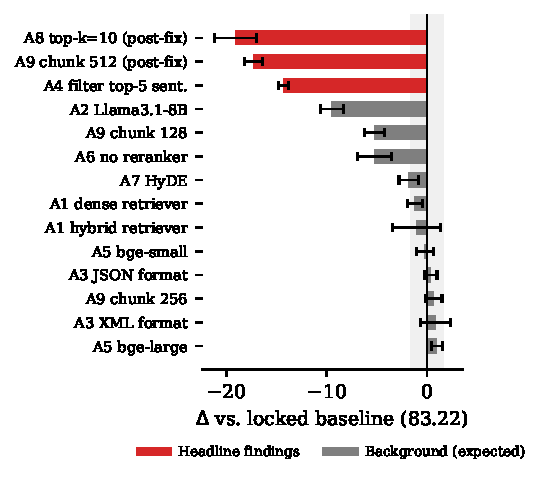
\includegraphics[width=\columnwidth]{fig2_ablation_deltas.pdf}
  \caption{$\Delta$ from locked baseline across conditions, ordered by magnitude.
  Headline findings (red) exceed the $\pm$1.52 noise band (shaded); background findings (gray) confirm expected effects.}
  \label{fig:deltas}
\end{figure}

\section{Conclusion}

Faithful RAG evaluation requires checking not only whether models ground answers in retrieved text, but whether the evaluation stack itself fails silently.
We found an LLM judge that returns valid zeros above a context threshold, a post-reranking filter that destroys grounding despite perfect retrieval, and a recall metric that certifies success at document level while the answer-bearing passage is unavailable.
These issues surfaced only because we ran replicated ablations at scale and audited anomalous scores rather than accepting them as pipeline failure.
Code and data: anonymized repository (link upon acceptance).

\section*{Limitations}
\label{sec:limitations}

Each condition uses $n{=}3$ replications; we report means and standard deviations but cannot claim statistical significance---only direction and magnitude.
The 60 questions were written by the pipeline author over a self-selected paper set, a convenience benchmark we acknowledge openly.
Our judge model changed during early development (Llama3.1-8B $\rightarrow$ Qwen2.5-14B); all reported ablations use the fixed later regime.
Findings describe one local pipeline and one academic-QA corpus; we expect the \emph{qualitative} patterns---silent judge failure, filter--reranker interaction, passage-level recall gaps---to generalize to other setups using LLM judges and document-level metrics, but not necessarily the exact point deltas.
No human subjects or sensitive data were involved.

\bibliography{custom}

\end{document}
